\chapter[Solução]{Solução}\label{cap2}

\section{Solução de Energia}
O grupo de engenharia de energia é responsável pela análise e escolha da fonte energética do projeto, pelo estudo do tempo de duração da carga desta fonte, bem como o dimensionamento do sistema fotovoltaico offgrid a ser instalado.


\subsection{Motor}
Neste projeto será utilizado o motor elétrico, que é uma máquina de construção simples,e que possui uma grande versatilidade de adaptação às cargas dos mais diversos tipos e potências.

Entre os tipos de motores estão os de corrente alternada e os de corrente contínua. Foi escolhido o de corrente contínua, pois apesar do seu custo mais elevado, ele funciona com velocidade ajustável entre amplos limites e se prestam a controles de grande flexibilidade e precisão.

\subsubsection{Dimensionamento do Motor}

Para a definição de capacidade de dosagem do sistema de dosagem, utilizou-se a equação abaixo \cite{agricola}:

\begin{equation}
Q=4,71.10^{-5}.(D^{2}-d^{2}).p.n
\end{equation}

Onde:


D = diâmetro da rosca tubular, cm;

Q = capacidade, $m³/h$;

d = diâmetro interno do helicóide, cm;

p = passo do helicóide, cm e

n = rotação, rpm.

\begin{equation}
Q=4,71.10^{-5}.(10^{2}-2,5^{2}).10.28
\end{equation}

Cálculo da potência requerida:

\begin{equation}
Pt = 2,22.10^{-4}.(Q.\mu.L.\emptyset)
\end{equation}

Onde:

Pt = potência requerida pelo transportador, cv;

Q = capacidade, $m^3/h$;

$\mu$ = massa específica do material, $kg/m^3$;

L = comprimento total do transportador, m e

$\emptyset$ = fator de potência adimensional.


\begin{equation}
Pt = 2,22*10^{-4}*(0,020605*243,66*1*0,4)
\end{equation}
\begin{equation}
Pt = 0,000447*2
\end{equation}
\begin{equation}
Pt = 0,0008941 \text{CV}
\end{equation}


A potência é multiplicada por 2, pois quando seu valor é menor que 1,0 , deve-se aplicar o fator de correção no valor de 2.

Cálculo do torque:

\begin{equation}
T=9550.\frac{Pt}{n}
\end{equation}

Onde:

T = torque, N.m;

Pt = potência requerida pelo transportador, kW;

Logo, o tem-se um torque requerido de $T=0,2017N.m$

\subsubsection{Motor DC}

O motor escolhido foi o da marca Bosh, modelo F006 B20 321, e foi acoplado à rosca helicoidal, como mostra a figura abaixo.

\begin{figure}[!h]
\centering 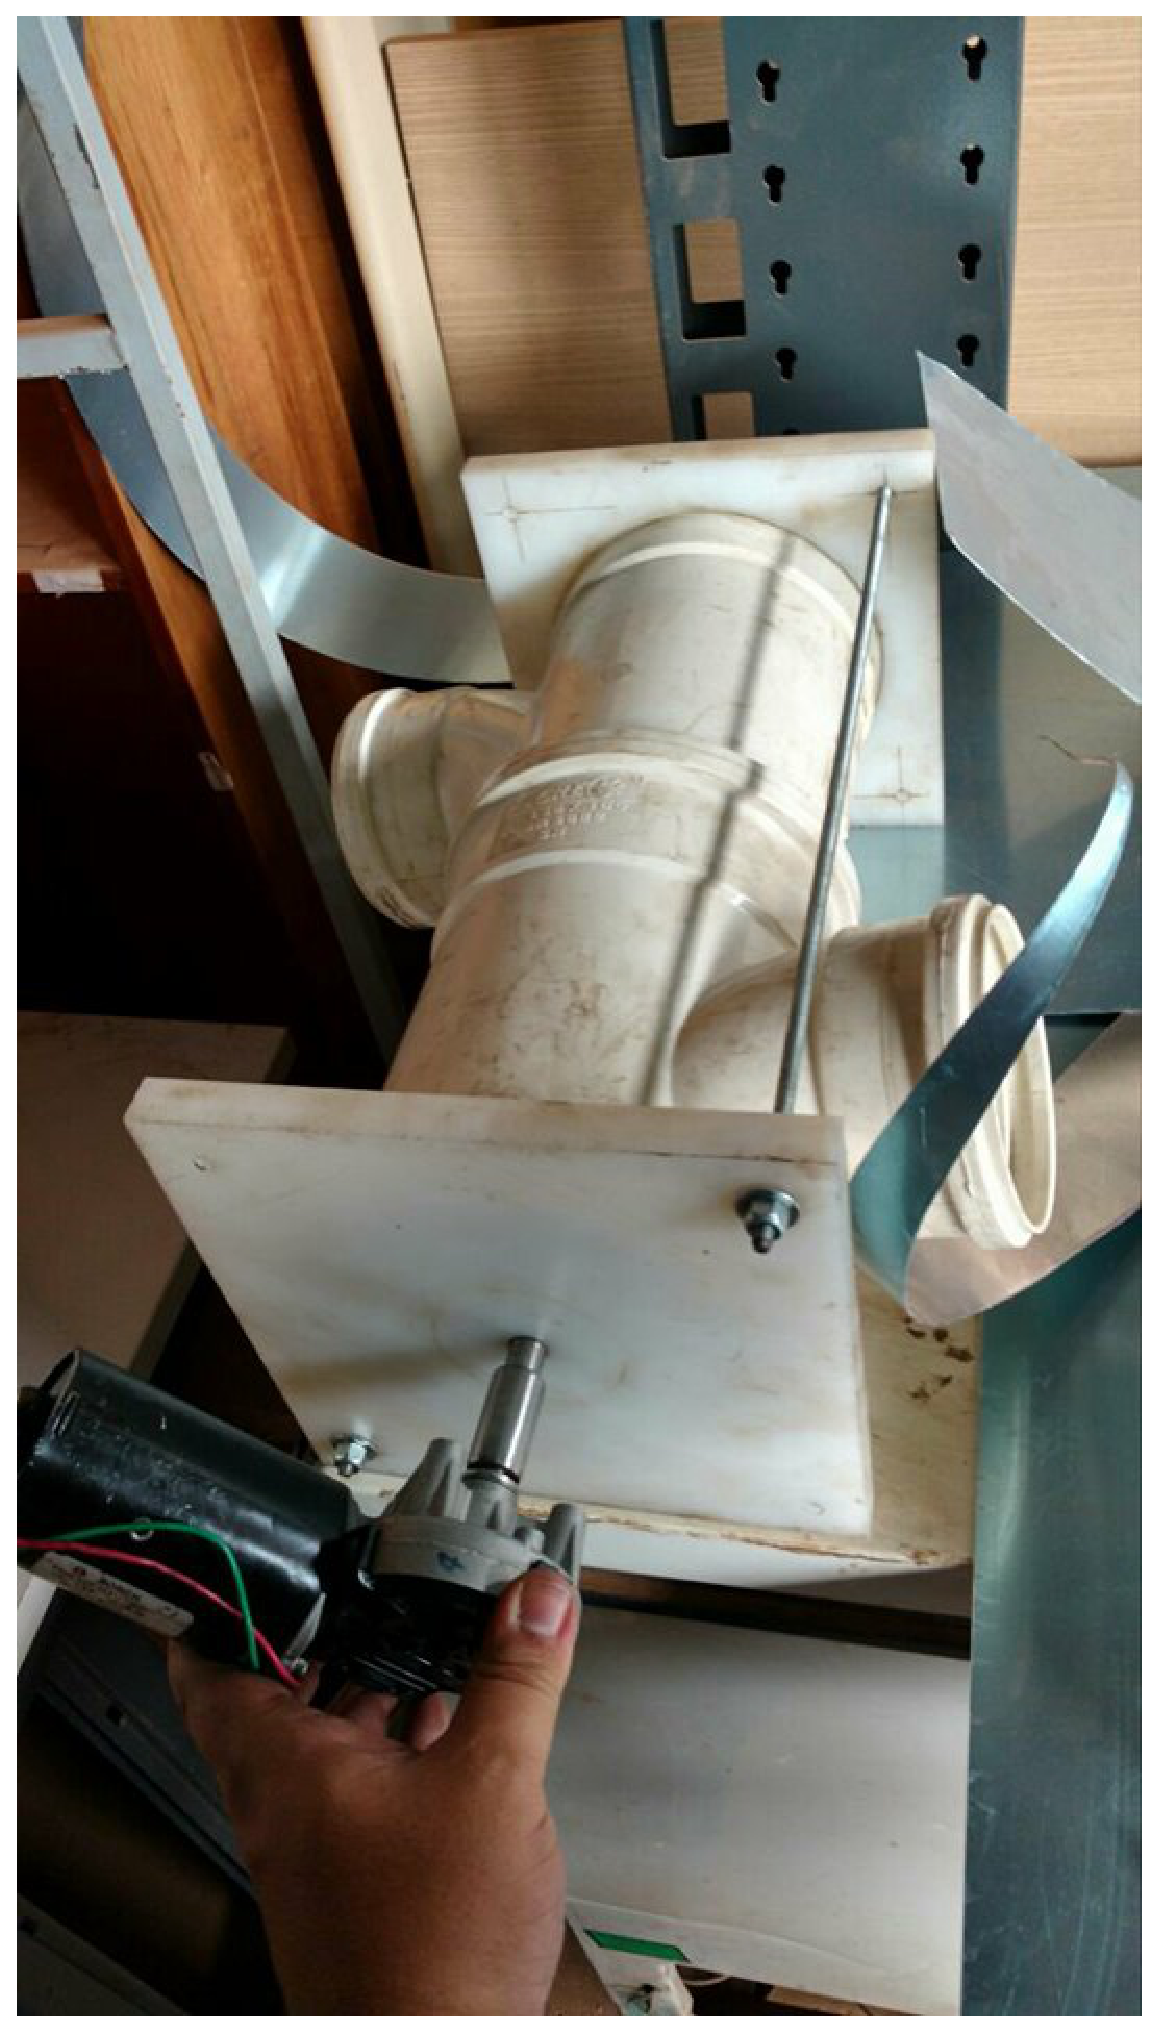
\includegraphics[scale=0.3]{figuras/motor}
\caption{Motor acoplado à rosca helicoidal}
\label{motor}
 \end{figure}

\subsection{Sistema de Alimentação de Energia}
O sistema de alimentação de energia será por meio de placa fotovoltaica, visto que o alimentador de peixes ficará no meio do lago, e não será possível fazer recarga de bateria. O sistema de geração é composto por:

\begin{itemize}
    \item Painel Solar Fotovoltaico
    \item Bateria
    \item Controlador de Carga
    \item Cabos para conexão do equipamento
    \item Suporte para o painel fotovoltaico



\end{itemize}

\subsubsection{Dimensionamento Sistema Fotovoltaico}
A grande vantagem da utilização da energia solar no projeto, é que esta é uma fonte renovável e sustentável. Além disso, o sistema tem um baixo custo de manutenção e longa vida útil. Quando houver energia excedente, a energia será armazenada na bateria estacionária. A seguir serão apresentados alguns dados necessários para o dimensionamento e o cálculo do número de módulos a ser utilizado no sistema.


\subsubsection*{Insolação}

A insolação da região de Dianópolis foi consultada no site da CRESESB, com valor médio de 4,94 Wh/$m^{2^{}}$/dia.

\subsubsection*{Consumo diário do sistema}
O cálculo do consumo consiste na quantidade de watt-hora utilizada pelo motor e pelos componentes eletrônicos:
\\

$19~W*3h~=57~Wh/dia~\rightarrow~\text{Motor}$

$2~W*24h~=48~Wh/dia~\rightarrow~\text{Eletrônica}$
\\

Portanto, o valor total de consumo do sistema é de $57+48=105~Wh/dia$, ou 0,105 kWh/dia.

\subsubsection*{Características da Placa}
Informações como área, eficiência e potência da placa foram retiradas do próprio fabricante Yingli e podem ser observadas na tabela a seguir.

\begin{table}[!ht]
\centering
\caption{Características da Placa Fotovoltaica Yingli}
\label{my-label}
\begin{tabular}{|c|c|c|}
\hline
\textbf{Potência} & \textbf{Eficiência} & \textbf{Área} \\ \hline
30 W & 15\% & 0,2652 $m^{2}$ \\ \hline
\end{tabular}
\end{table}

\subsubsection*{Cálculo do número de módulos}
O número de módulos/placas que o sistema necessitará é calculado a partir da fórmula a seguir:


\begin{equation}
N_{\text{módulo}}= \frac{\text{Consumo por dia}}{\text{Insolação}\times~\text{Eficiência}~\times\text{Área da placa}}
\end{equation}

Onde:
\begin{equation}
N_{\text{módulo}}= \frac{0,105}{4,94\times0,15\times0,262} = 0,54
\end{equation}

Pelo cálculo acima, pode-se afirmar que a placa escolhida para o projeto é suficiente para suprir a demanda do sistema.

\subsubsection{Bateria}

Será necessária a utilização de uma bateria como de alimentação de motores e componentes eletrônicos do projeto, devido à incapacidade na utilização de energia elétrica e na praticidade ao utilizar a energia solar já disponível no local.

A bateria é utilizada nos sistemas fotovoltaicos para armazenar energia excedente produzida pelos painéis, para ser utilizada durante a noite ou em dias nublados ou com baixa insolação. As mais utilizadas em sistemas de energia renovável são as do tipo estacionárias ou de ciclo profundo, pois suportam grandes descargas que uma bateria comum não suportaria.


\begin{itemize}
\item{Dimensionamento da Bateria}
\end{itemize}

Conforme a potência total requerida pelo sistema (motor + componentes eletrônicos), 19 W + 2 W, calculou-se a corrente necessária.

Cálculo da corrente:

\begin{equation}
P_\text{motor}=19~W
\end{equation}

\begin{equation}
P_\text{eletrônica}=2~W
\end{equation}

\begin{equation}
P_{total}=P_\text{motor}+P_\text{eletrônica}=21~W
\end{equation}

\begin{equation}
i=\frac{P}{V}
\end{equation}

\begin{equation}
i\text{(motor)}=\frac{19}{12} = 1,58\,A
\end{equation}

\begin{equation}
i\text{(eletrônica)}=\frac{2}{12} = 0,166\,A
\end{equation}

Considerando a autonomia de 3h para o motor, e 24h para os componentes eletrônicos, calculou-se a capacidade da bateria.

\begin{equation}
\text{Capacidade}=(1,58\times3h).(0,166\times24h)=8,74~Ah
\end{equation}

Assim, a capacidade da bateria é 8,74 Ah, porém não é recomendado a descarga total, devido reduzir a vida útil da bateria. Considerando uma descarga de 75\%, calculou-se a capacidade para bateria.

Cálculo Capacidade da Bateria:

\begin{equation}
Ah=\frac{8,74\,Ah}{0,75}
\end{equation}

\begin{equation}
Ah=11,65
\end{equation}

Através do dimensionamento realizado a partir dos cálculos mostrados acima, foi escolhido uma bateria de 12Ah, como mostram as figuras abaixo:

% \begin{figure}[!ht]
% \centering
%     \subfigure [a]{
%         \includegraphics[keepaspectratio=true,scale=0.15]{figuras/bateria1}
%         \label{Figura3} %esse é o nome da figura (a)
%     }
%     \qquad
%     \subfigure[b]{
%         \includegraphics[keepaspectratio=true,scale=0.15]{figuras/bateria2}
%         \label{Figura4} %esse é o nome da figura (b)
%     }\\
%
%    \caption{Bateria}
% \label{figuras1}
% \end{figure}

\begin{figure}[h]
\centering
\includegraphics[keepaspectratio=true,scale=0.15]{figuras/bateria1}
\caption{Bateria}
\label{Figura3}
\end{figure}

\begin{figure}[h]
\centering
\includegraphics[keepaspectratio=true,scale=0.15]{figuras/bateria2}
\caption{Bateria}
\label{Figura4}
\end{figure}

\subsubsection{Controlador de Carga}
Será utilizado um controlador de carga acoplado aos painéis
fotovoltaicos e a bateria para realizar o controle e proteção do sistema.O controlador é responsável pela duração da vida útil dos bancos de baterias protegendo-o contra sobretensões e descargas excessivas. Assim, é de fundamental importância a utilização de um controlador de cargas. Esses controladores se localizam entre painéis fotovoltaicos e baterias onde controla-se a tensão de entrada já que as baterias não suportam grande flutuação de energia. Sendo assim, permite que as baterias sejam carregadas de melhor forma informando o estado de carga da bateria \cite{serrao2010dimensionamento}.
Para o dimensionamento do controlador, utiliza-se o consumo total do sistema (105 Wh) e a tensão da bateria (12V):

\begin{equation}
CC=\frac{105~Wh}{12~V}
\end{equation}

\begin{equation}
CC=8,75~A
\end{equation}

Conforme o cálculo acima, foi escolhido um controlador de carga de 10A, mostrado nas figuras abaixo:

\begin{figure}[h]
\centering
\includegraphics[keepaspectratio=true,scale=0.15]{figuras/controlador1}
\caption{Bateria}
\label{Figura3}
\end{figure}

\begin{figure}[h]
\centering
\includegraphics[keepaspectratio=true,scale=0.15]{figuras/controlador2}
\caption{Controlador de carga}
\label{Figura4}
\end{figure}

% \begin{figure}[!htb]
% \centering
%     \subfigure [a]{
%         \includegraphics[keepaspectratio=true,scale=0.15]{figuras/controlador1}
%         \label{Figura3} %esse é o nome da figura (a)
%     }
%     \qquad
%     \subfigure [b]{
%         \includegraphics[keepaspectratio=true,scale=0.15]{figuras/controlador2}
%         \label{Figura4} %esse é o nome da figura (b)
%     }\\
%
%    \caption{Controlador de carga}
% \label{figuras1}
% \end{figure}


    Características do controlador de carga solar SR 10A HP2410 – PWM:

    \begin{itemize}
\item{Identificação automática de sistemas de tensão 12/24V;}
\item{Visor LED digital com um sistema de interação simplificado, tornando seu manuseio simples e conveniente;}
\item{Estende a vida útil da bateria através da sua tecnologia de algoritmo de ponta.}
\item{Possuí quatro modos operacionais;}
\item{Alta durabilidade, podendo ser utilizado em ambientes hostis;}
\item{Saída 5V para USB, pode ser usada para carregar equipamentos eletrônicos como o celular;}
\item{Possui diversos tipos de indicações de status;}
\item{Periodicamente ou quando detectado descarregamento profundo da bateria, o controlador opera em modo equalizador, de forma a evitar sulfuração e desbalanceamento da bateria, o que aumenta efetivamente sua vida útil.}

\end{itemize}



\subsection{Dimensionamento do Condutor}

\par O dimensionamento dos condutores consiste em determinar a seção mínima de forma que suportem simultaneamente o aquecimento excessivo e a queda de tensão durante a passagem da corrente.Essa atividade visa garantir uma vida satisfatória aos condutores e isolações quando submetidos aos efeitos térmicos produzidos pela circulação de correntes.
\par De acordo com a NBR 5410 o dimensionamento de um condutor se inicia com a escolha do tipo de isolação que determina a temperatura máxima em regime contínuo,sobrecarga e curto-circuito. A tabela 35 da página 100 da NBR 5410 está representada abaixo.




\begin{table}[h]
\centering
\caption{Temperaturas características dos condutores}
\label{my-label}
\begin{tabular}{|c|c|c|c|}
\hline
Tipo de isolação                                                                                         & \begin{tabular}[c]{@{}c@{}}Temperatura max. \\ para serviço\end{tabular} & \begin{tabular}[c]{@{}c@{}}Temp. limite de \\ sobrecarga\end{tabular} & \begin{tabular}[c]{@{}c@{}}Temp. limite de \\ curto-circuito\end{tabular} \\ \hline
\begin{tabular}[c]{@{}c@{}}Policloreto de vinila (PVC)\\  até 300 mm\textasciicircum 2\end{tabular}      & 70                                                                       & 100                                                                   & 160                                                                       \\ \hline
\begin{tabular}[c]{@{}c@{}}Policloreto de vinila (PVC)\\ maior que 300 mm\textasciicircum 2\end{tabular} & 70                                                                       & 100                                                                   & 140                                                                       \\ \hline
\begin{tabular}[c]{@{}c@{}}Borracha etileno-propileno \\ (EPR)\end{tabular}                              & 90                                                                       & 130                                                                   & 250                                                                       \\ \hline
\begin{tabular}[c]{@{}c@{}}Polietileno reticulado\\  (XLPE)\end{tabular}                                 & 90                                                                       & 130                                                                   & 250                                                                       \\ \hline
\end{tabular}
\end{table}
\par Logo, o melhor tipo de isolação para este projeto é a isolação PVC até 300 mm$^2$.
\par Após a escolha do tipo de isolação é feita a classificação quanto à forma de utilização, se é ao ar livre ou passando por eletrodutos, no caso os cabos não estarão passados por um eletroduto, ficarão ao ar livre, sendo classifido então no método de referência F e no método de instalação (Tabela 33 da NBR 5410) número 13.
\par Em seguida calculamos a corrente de projeto para então determinar a melhor bitola para a instalação.
\begin{equation}
I_p= \frac{P}{V}
\end{equation}
\begin{equation}
I_p= \frac{19}{12}=1,6 A
\end{equation}

\par Onde, a potência que foi utilizada para o cálculo é a potência do motor, pois os cabos serão direcionados diretamente da bateria para o motor, nenhuma outra carga será conectada a este cabo.
\par Então conhecidos os números de condutores, que no caso para este projeto são apenas 2 condutores carregados. Com este valores da referência (F), corrente de projeto e número de condutores é consultada a Tabela 38 da NBR 5410 (página 103) para a definição da seção do fio necessária para alimentação do motor. Logo, foi verificado que a seção 0,5 mm $^2$ é suficiente, pois atende uma corrente de até 2A.

\par Os fios elétricos são especificados por um número, em função da carga elétrica por eles suportável. De acordo com a NBR 5410 da ABNT, podemos dimensionar a bitola do fio condutor da seguinte maneira:
\begin{equation}
s= \frac{L*P}{\sigma \times e\times {U}^{2}}
\end{equation}

\par Os fatores que influênciam no dimensionamento da bitola do fio a ser utilizado em um projeto são: a distância que a corrente elétrica tem de percorrer ao longo do fio (dada em metros), a potência do sistema (dada em Watts), a queda de tensão (considerada de 3\% para sistemas CC e 5\% para sistemas AC), a tensão de trabalho (V) e a condutividade elétrica dos cabos (condutividade elétrica do cobre é 56 metros por ohms milimetros ao quadrado).

\begin{equation}
s= \frac{2*129}{56 \times 0,03\times {12}^{2}}
\end{equation}
\par Logo a bitola do fio necessária para suportar o sistema é de:
\begin{equation}
s= 1,06 mm^2
\end{equation}
\par Então o condutor mais indicado para este projeto seria o condutor com bitola de no mínimo 1,5 mm, pois é o condutor com seção comercializada que vem logo acima do valor da capacidade calculada. Este condutor suporta uma corrente de até 15 amperes sem aquecer.
\par A capacidade de condução de energia de um condutor pode ser definida como  a maior corrente, em regime permanente, que ele suporta sem que a temperatura do mesmo ultrapasse a temperatura máxima suportada pela isolação.
\par O dimensionamento incorreto, resulta na diminuição da eficiência e no sobreaquecimento do fio que devido à elevação da temperatura diminui a sua capacidade de condução de corrente. E como consequência, pode resultar em curto-circúito, perigo de choques e incêndio.

\subsection{Sistema de Proteção}

\par Os dispositivos de proteção são componentes que, inseridos nos circuitos elétricos, servem para proteção do circuito elétrico e dos dispositivos e equipamentos presentes, como por exemplo, motores, CLP’s, tornos, etc. Estas proteções interrompem a circulação de corrente quando alguma anomalia acontece, como um curto circuito ou uma descarga atmosférica.
\par O aumento da temperatura nos condutores de uma instalação elétrica, devido a circulação de corrente (efeito Joule), projetada para o funcionamento normal, deve ser limitado para não prejudicar os elementos.
\par A proteção do sistema de alimentação será realizada com a utilização de fusíveis que são dispositivos simples que servem como proteção de circuitos elétricos bem como equipamentos. Ele pode ser encontrado em instalações elétricas de baixa tensão aonde protege cargas como por exemplo lâmpadas e até mesmo em sistemas complexos de geração e distribuição de energia, por seu baixo custo e modo de operação simples.
\par Os fusíveis contêm um elemento condutor constituído de uma liga metálica especial, dimensionado para fundir, sob o aquecimento resultante do efeito joule, quando submetidos a correntes maiores que um valor especificado, que é a corrente nominal do fusível. Quanto maior a corrente circulante diante da nominal, menor será o período de tempo para a fusão.
\par Os fusíveis podem ser classificados de acordo com as seguintes codificações: gL, gG, aM e aR, que tem o seguinte significado: as letras minúsculas representam a faixa de interrupção, ou seja, com que tipo de sobrecorrente que o fusível irá atuar, sendo "g"- atuação para sobrecarga e curto e "a"- atuação apenas para curto-circuito. E as letras maiúsculas significam a categoria de utilização, ou seja, para que tipo de equipamento o fusível é indicado: sendo "L"- Proteção e uso de cabos geral; "G"- Proteção e uso de cabos geral; "M"- Proteção de Motores; e "R"- Proteção de circuitos com semicondutores.
\par Para proteger o circuito do motor do fuso foram realizados os seguintes cálculos para dimensionar a corrente que o fusível deve suportar sem fundir.

\par Logo, o fusível cujo valor de corrente deve ser maior do que a corrente nominal que o motor pode drenar em funcionamento normal, ou seja, como a corrente nominal que pode circular no circuito bateria-motor é de 4,5A,  é calculada uma margem de segurança de 1,5 vezes o valor da corrente nominal do motor, o que resulta na escolha de um fusível 6A aM, ou seja, para atuar como proteção do motor em caso de curto-circuito.
\par Para o sistema de prteção dos componentes eletrônicos foi desenvolvido o mesmo cálculo, porém substituindo o valor da potência por 2W.
\begin{equation}
i\text{(eletrônica)}=\frac{2}{12} =166 mA
\end{equation}

\par Logo, o fusível cujo valor de corrente deve ser maior do que a corrente nominal que os componentes eletrônicos pode drenar em funcionamento normal, ou seja, como a corrente que circula no circuito bateria-componentes eletrônicos é de 166 mA,  é calculada uma margem de segurança de 1,5 vezes o valor dessa corrente, o que resulta na escolha de um fusível de 250 mA aM, ou seja, para atuar como proteção dos componentes em caso de curto-circuito.


\begin{figure}[!h]
\centering
\includegraphics[scale=0.2]{figuras/fusivel}
\caption{Fusível em cilindro de vidro e seu suporte}
\label{fusivel}
\end{figure}
\par Na imagem abaixo está representada a placa com os componentes eletrônico e os dois fusíveis para a proteção de todo o sistema elétrico.

\begin{figure}[!h]
\centering
\includegraphics[scale=0.2]{figuras/placa-fusivel}
\caption{Fusíveis instalados na placa eletrônica}
\label{fusivel}
\end{figure}
\pagebreak

\subsection{Suporte da Placa Fotovoltaica}

O suporte da placa fotovoltaica, como é mostrado nas figuras abaixo, foi feito utilizando dois apoios com cantoneira de aluminio, deixando a placa a uma angulação de 14 graus, pois é a angulação da latitude da cidade de Dianópolis-TO. A placa foi parafusada no suporte, e a cantoneira fixada por rebites na tampa da estrutura.

\begin{figure}[!h]
\centering
\includegraphics[scale=0.3]{figuras/placa}
\caption{Vista lateral da placa fixada na tampa}
\label{placa}
\end{figure}

\begin{figure}[!h]
\centering
\includegraphics[scale=0.3]{figuras/placa1}
\caption{Vista lateral da placa fixada na tampa}
\label{placa1}
\end{figure}
